\documentclass[12pt]{article}
\usepackage{amsmath,amsfonts}
\usepackage{enumerate}
\usepackage{graphicx}
\usepackage{float}
\usepackage{multirow}
\usepackage{booktabs}

\renewcommand{\baselinestretch}{1}
\topmargin 0in \headheight 0.0in \textheight 9in \textwidth 6.5in
\oddsidemargin 0.1in \evensidemargin 0.1in

\graphicspath{{/Users/siyangren/Documents/ra-cida/ESFGSP_Paper/Simulations/results/figures}}


\begin{document}

\section*{Methods}

In this study, we conducted two simulations to evaluate the performace of LASSO models in identifying significant
features within high-dimensional datasets. The first simulation assumes sparsity in the feature space corresponding to
pixels, referred to as the pixel space, while the second simulation assumes sparsity in the frequency domain, known as
the frequency space. The pixel space represents the original high-dimensional domain, where each dimension corresponds
to a pixel in an image. Features in this space are directly observable and may exhibit inherent correlations. In
contrast, the frequency space is a transformed version of the pixel space, derived through eigen decomposition, where
the data is represented in terms of its frequency components.

Let \( X \) denote a column vector representing the pixel values of a single observation, with 256 pixels in total. Its
covariance matrix, \( \Sigma \), is defined to have an exponential correlation structure, where \( \Sigma_{i j}=-\exp
(\operatorname{dist}(i, j)) \). Here, \( \operatorname{dist}(i, j) \) is the distance between the pixels \( i \) and \(
j \) in a \( 16 \times 16 \) grid. The matrix \( V \) contains the eigenvectors of \( \Sigma \), with each column
representing an eigenvector. We transform the random vector \( X \) into the frequency space by computing \( X_{\text
{freq }}=V^T X \). The covariance matrix of \( X_{\text {freq }} \) is then given by \(
\operatorname{cov}(X_{\mathrm{freq}})=V^T \Sigma V \), which results in a diagonal matrix.

In each simulation iteration, 1000 observations of \( X_{\text {freq}} \) are generated from a multivariate normal
distribution with the covariance matrix \(\operatorname{cov}\left(X_{\text {freq }}\right) \). This process is repeated
across 500 iterations.  For each observation, we compute the corresponding pixel space vector \( X \) as \( X=V X_{\text
{freq }} \).

In the first simulation, we assume that the coefficient vector \( \beta \) is sparse in the pixel space. Specifically,
the non-zero values in \( \beta \) are confined to a central \( 8 \times 8 \) region of the image. The response variable
\( y \) is drawn from a binomial distribution, with the success probability determined by \( \eta = X \beta \). The
non-zero coefficients in \( \beta \) are chosen to ensure that the probability \( p = \frac{1}{1 + \exp(-\eta)} \) is
uniformly distributed within the interval \( [0, 1] \).

In the second simulation, sparsity is assumed in the coefficient vector \( b \) within the frequency space. Here, 10\%
of the 256 entries in \( b \) are randomly set to non-zero values, while the rest remain zero. The response variable \(
y \) is generated similarly to the first simulation, ensuring that the probability \( p \) is uniformly distributed. 

For both simulations, two models are fitted: one using the covariates in the pixel space and the other using the
covariates in the frequency space. Each dataset, consisting of 1000 observations with 256 features (representing \( 16
\times 16 \) pixel images), is split into training (80\%) and test (20\%) sets. The regularization parameter \( \lambda
\) is tuned using cross-validation based on the binomial deviance metric. The dataset is divided into 10 folds, with the
model trained and validated iteratively across these folds while varying \( \lambda \). We consider two specific \(
\lambda \) values, `lambda.min` which minimizes the cross-validated error, and `lambda.1se`, which represents the
largest \( \lambda \) within one standard error of the minimum.

After selecting the optimal \( \lambda \), model performance is assessed using accuracy and AUC (Area Under the Curve)
metrics. Additionally, a permutation test is conducted 100 times to calculate p-values for each covariate. Across all
iterations, we compute the mean and standard deviation of the metrics, as well as the percentage of significant p-values
for each covariate.  


\section*{Results}

In Simulation 1, the distribution of the success probability \( p \) was evaluated at various \( \beta \) values: 0.01,
0.05, 0.1, 0.2, and 1. As shown in Figure \ref{fig:sim1_p_dist}, \( \beta = 0.1 \) yielded the most uniform distribution
of \( p \), making it the optimal choice for model fitting. Similarly, in Simulation 2, the distribution of \( p \) was assessed at various \( b \) values: 0.1, 0.2, 0.4, 0.6, 0.8,
and 1. As illustrated in Figure \ref{fig:sim2_p_dist}, \( b = 0.4 \) resulted in the most uniform distribution of \( p
\). 

\begin{figure}[htbp] 
	\centering
	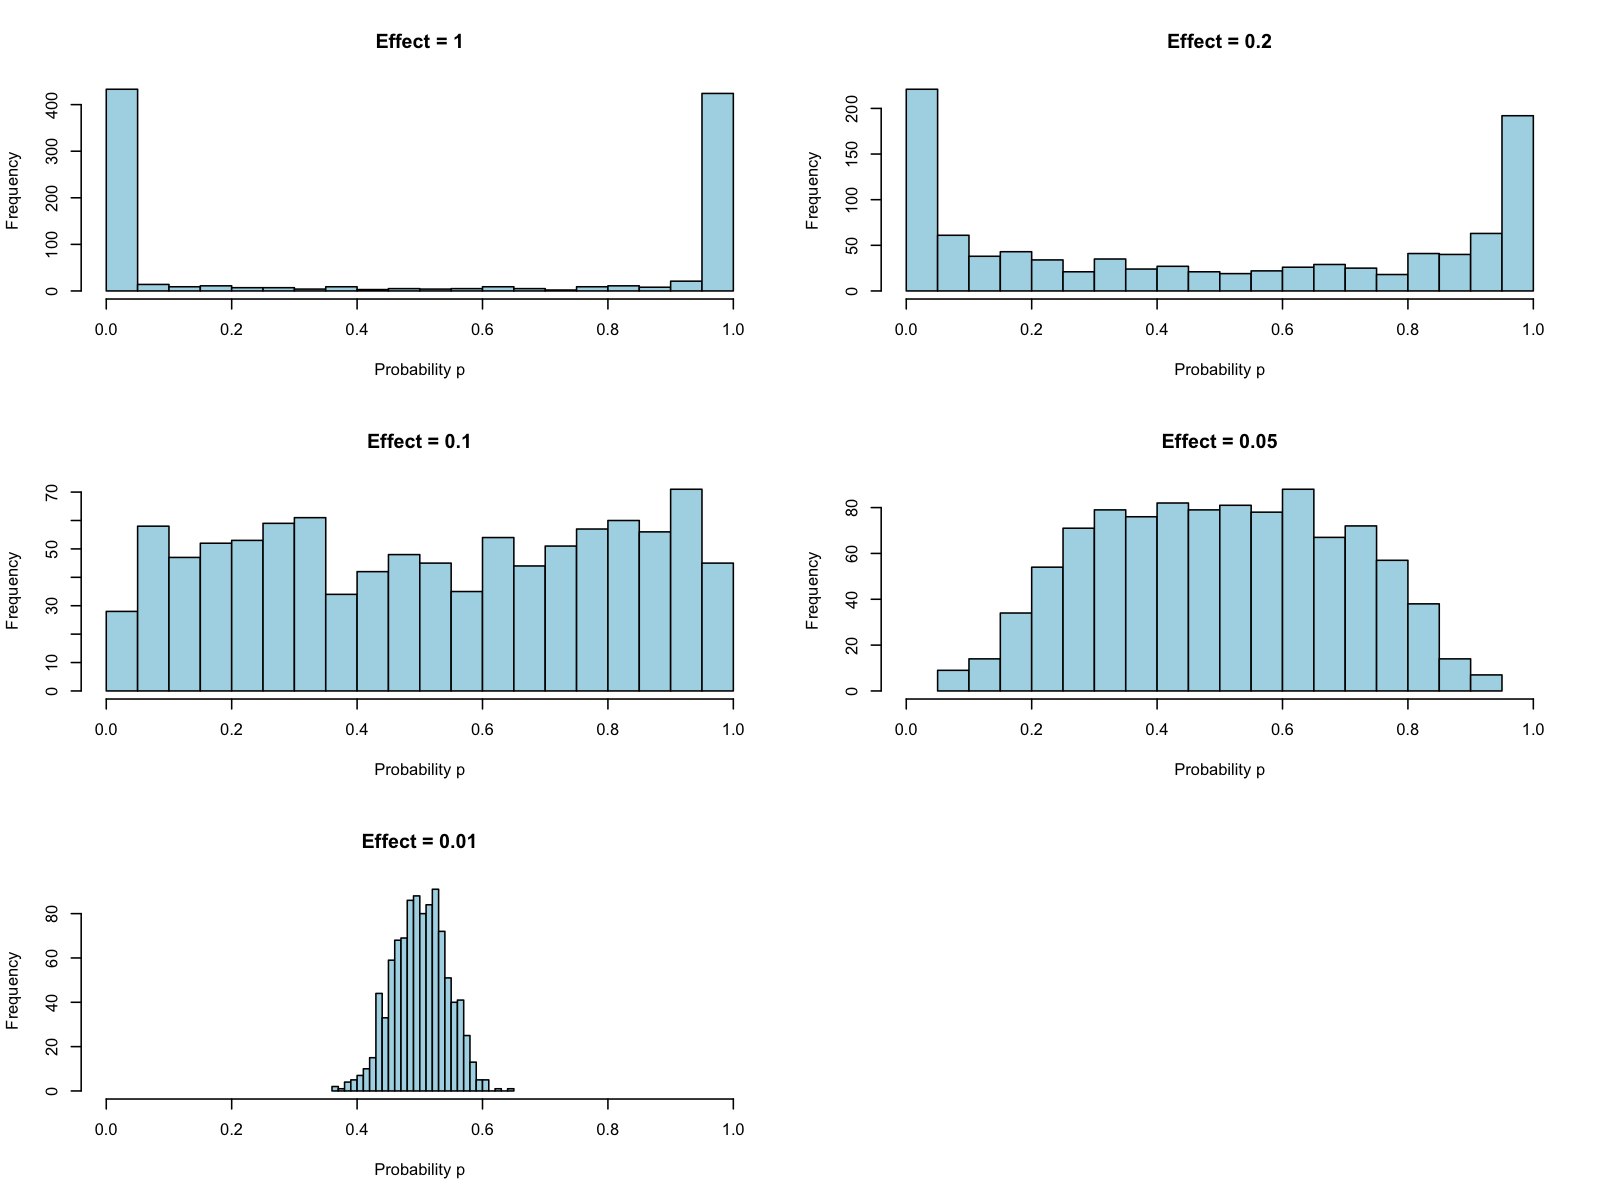
\includegraphics[width=0.9\textwidth]{sim1_p_dist.png} 
  \caption{Distribution of success probability \( p \) at different \( \beta \) values in Simulation 1.}
	\label{fig:sim1_p_dist} 
\end{figure}

\begin{figure}[htbp] 
	\centering
	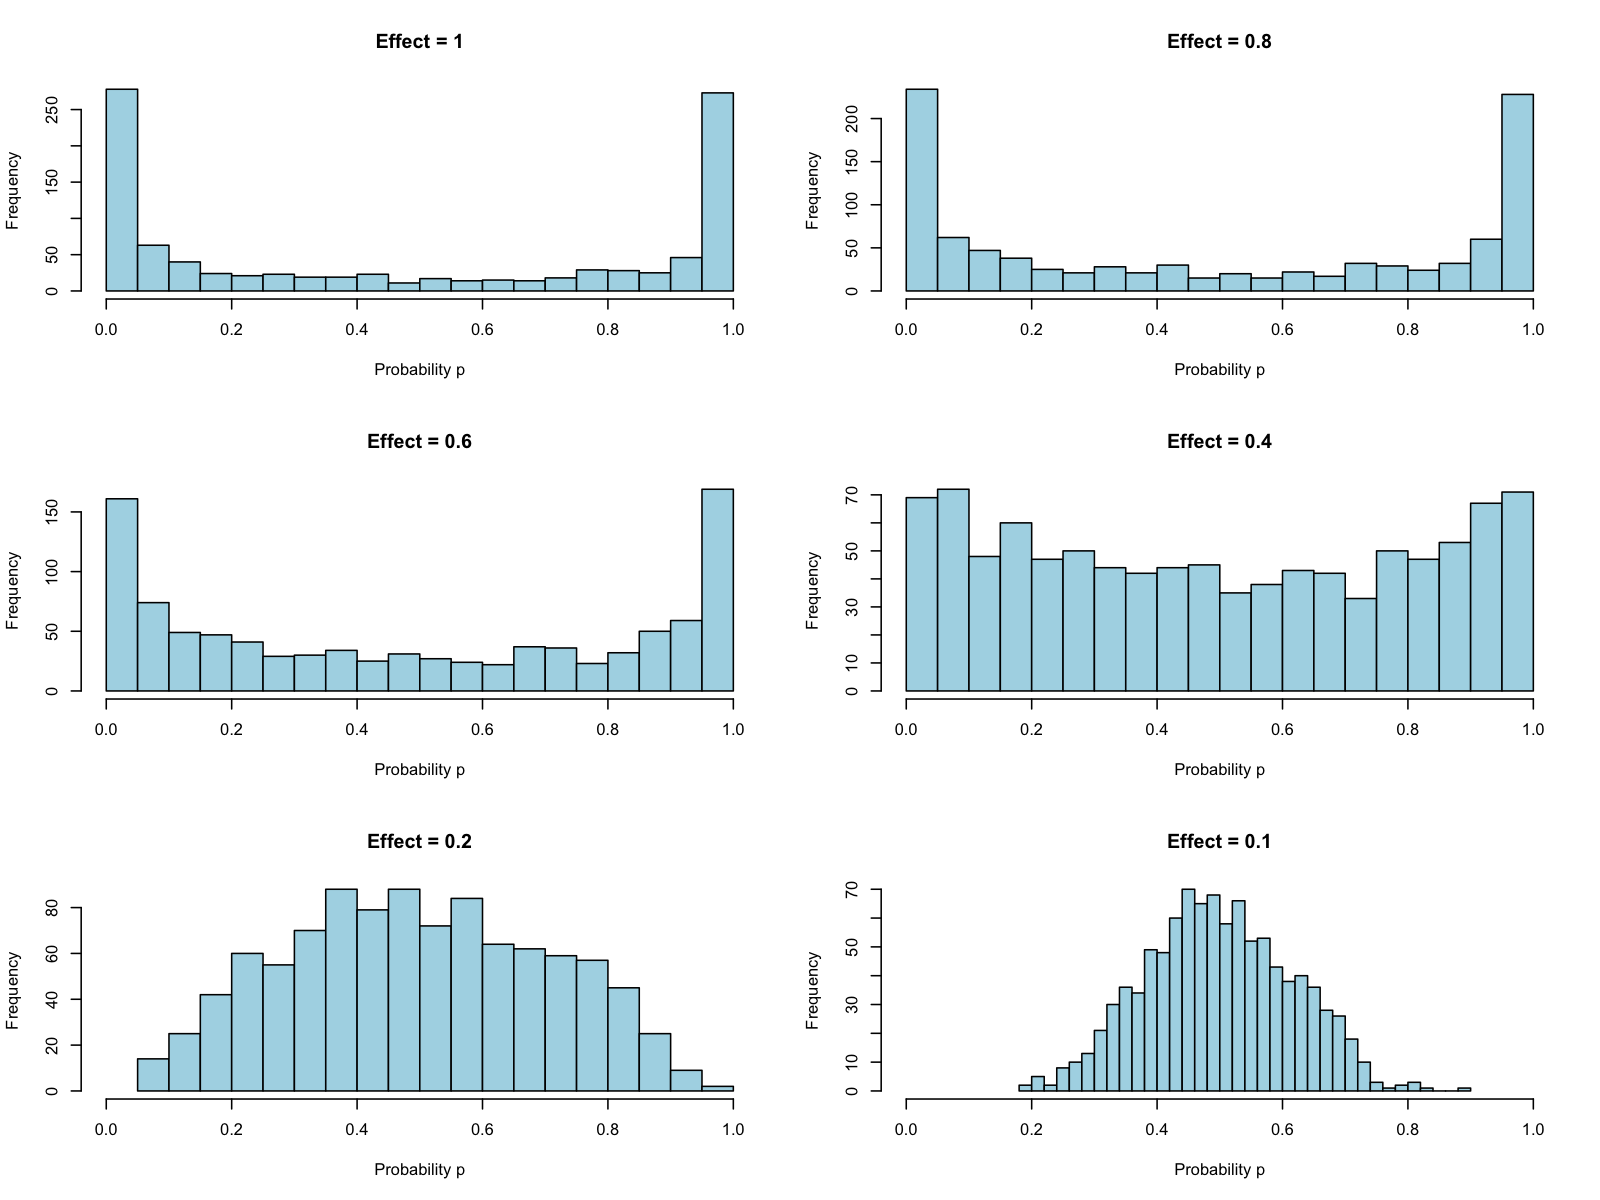
\includegraphics[width=\textwidth]{sim2_p_dist.png} 
  \caption{Distribution of success probability \( p \) at different \( b \) values in Simulation 2.}
	\label{fig:sim2_p_dist} 
\end{figure}

Using the selected values of \( \beta \) and \( b \), the response variable \( y \) was drawn from a binomial distribution with
success probabilities determined by \( \eta = X \beta \) in both simulations. Figure \ref{fig:group_diff1} and
\ref{fig:group_diff2} depict the group mean difference in covariate values between instances where \( y = 1 \) and \( y = 0
\) in both the pixel space and frequency space for Simulation 1 and 2, respectively. For Simulation 1, as shown in Figure \ref{fig:group_diff1}, the heatmap in the pixel space reveals that the central
region with non-zero coefficients in \( \beta \) corresponds to higher mean covariate values, which is consistent with
the heatmap of \( \beta \) in Figure \( \ref{fig:coefs_sim1} \). Similarly, regions with higher or lower values in the
frequency space match the corresponding values in the coefficients. A similar pattern is observed in Simulation 2, as illustrated in Figures \ref{fig:group_diff2} and \ref{fig:coefs_sim2},
where the heatmaps for both the pixel and frequency spaces demonstrate alignment between covariate values and the
corresponding non-zero coefficients. 

\begin{figure}[htbp] 
	\centering
	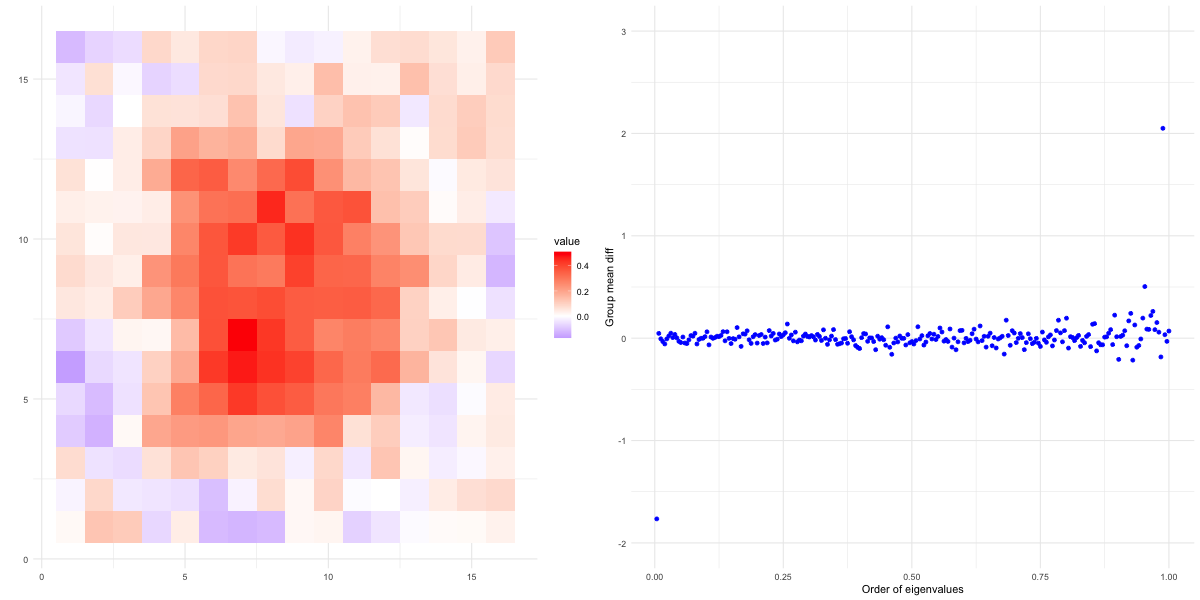
\includegraphics[width=0.9\textwidth]{group_mean_diff_sim1.png}
	\caption{Group mean difference in covariate values between instances where \( y = 1 \) and \( y = 0 \) in Simulation
  1, shown for both the pixel space (left) and frequency space (right).}
	\label{fig:group_diff1}
\end{figure}

\begin{figure}[htbp] 
	\centering
	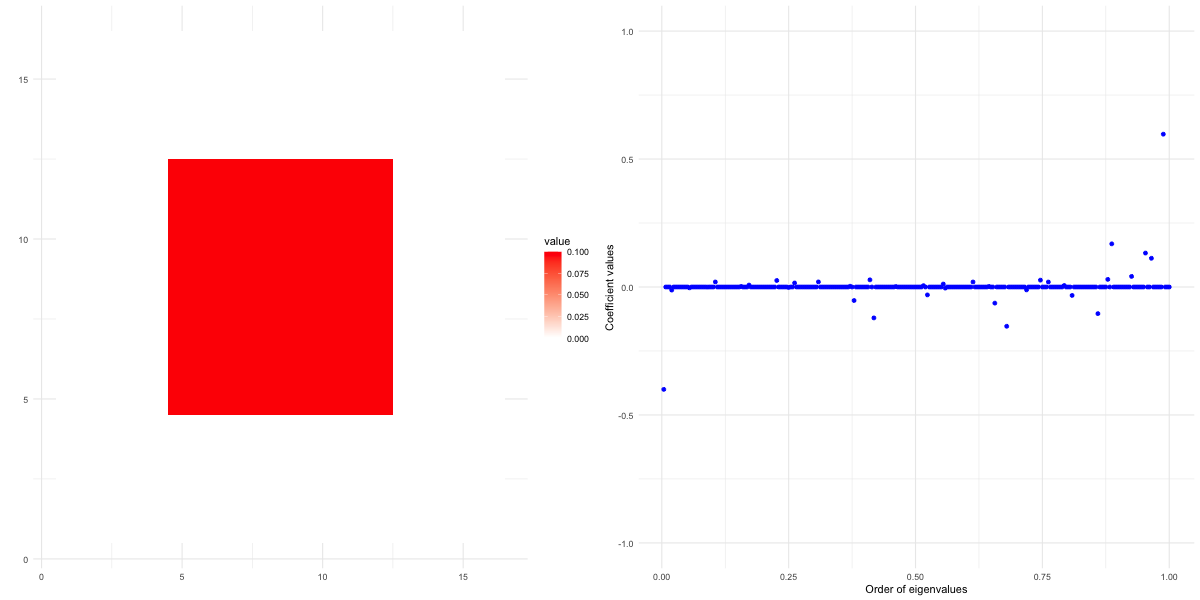
\includegraphics[width=0.9\textwidth]{actual_coefs_sim1.png}
  \caption{Actual coefficients in Simulation 1 for the pixel space (left) and frequency space (right).}
  \label{fig:coefs_sim1}
\end{figure}

\begin{figure}[htbp] 
	\centering
	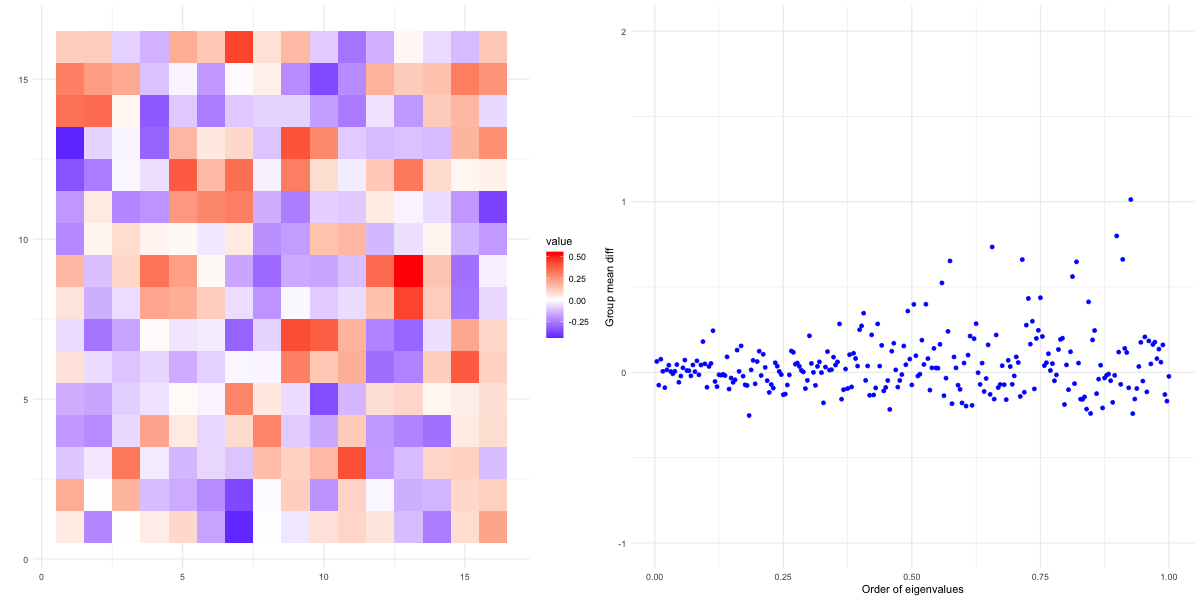
\includegraphics[width=0.9\textwidth]{group_mean_diff_sim2.png}
	\caption{Group mean difference in covariate values between instances where \( y = 1 \) and \( y = 0 \) in Simulation 2.}
	\label{fig:group_diff2}
\end{figure}

\begin{figure}[htbp] 
	\centering
	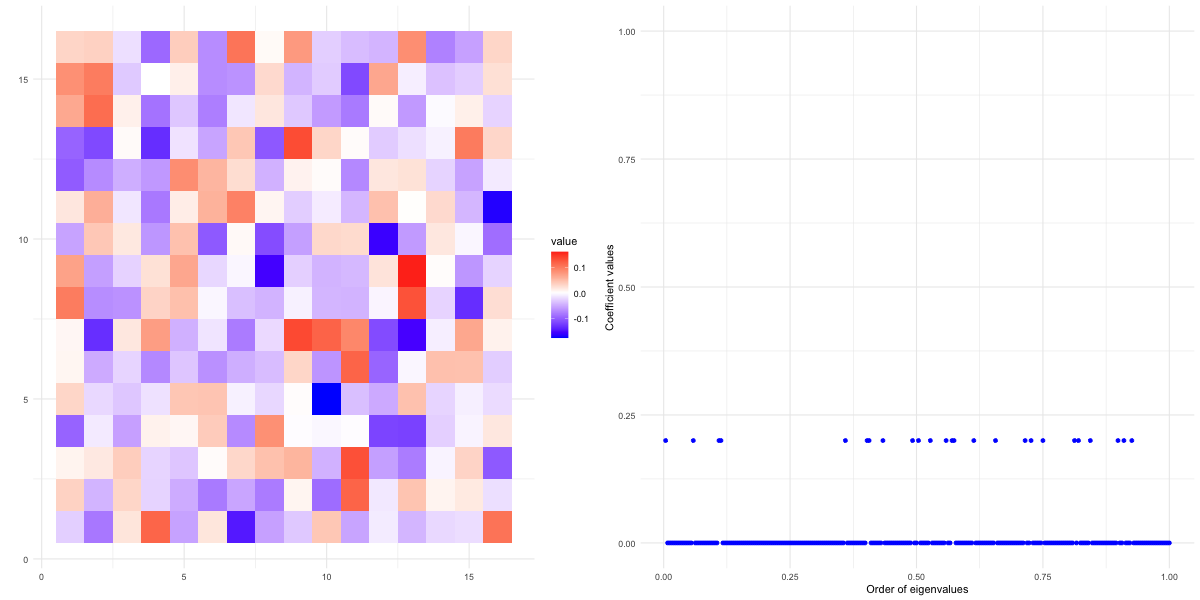
\includegraphics[width=0.9\textwidth]{actual_coefs_sim2.png}
  \caption{Actual coefficients in Simulation 2 for the pixel space (left) and frequency space (right).}
  \label{fig:coefs_sim2}
\end{figure}

To assess the performance of models fitted with covariates from the pixel space versus the frequency space, we evaluated
the area under the curve (AUC) and prediction accuracy. LASSO models were trained using cross-validation by splitting
each set of 1000 simulated observations into 80\% training and 20\% test sets. This process was repeated 500 times.
Table~\ref*{tab:auc_acc_table} presents the average AUCs and accuracies over the 500 iterations. Regardless of whether
sparsity is assumed in the pixel space (Simulation 1) or the frequency space (Simulation 2), models fitted in the
frequency space consistently outperformed those fitted in the pixel space. Specifically, in Simulation 1, using
`lambda.min` as the regularization value,  models fitted with covariates from the pixel space achieved an AUC of
0.803 (SE = 0.031) and an accuracy of 72.5\% (SE = 0.032). In contrast, models fitted with covariates from the 
frequency space achieved a slightly higher AUC of 0.827 (SE = 0.029) and a higher accuracy of
74.6\% (SE = 0.031). A similar trend was observed in Simulation 2, with models fitted in the frequency space
demonstrating superior performance regardless of the regularization parameter used.

\begin{table}[htbp]
\centering
\caption{Comparison of AUC and accuracy between models fitted in the pixel space and frequency space across 500 iterations for Simulation 1 and Simulation 2.}
\label{tab:auc_acc_table}
\begin{tabular}{l|cc|cc}
\toprule
\textbf{Simulation} & \multicolumn{2}{c}{\textbf{Model in Pixel Space}} & \multicolumn{2}{c}{\textbf{Model in Frequency Space}} \\ 
\midrule
& \textbf{AUC (SE)} & \textbf{Accuracy (SE)} & \textbf{AUC (SE)} & \textbf{Accuracy (SE)} \\ 
\midrule
\textbf{Simulation 1} & & & & \\
lambda.min & 0.803 (0.031) & 0.725 (0.032) & 0.827 (0.029) & 0.746 (0.031) \\
lambda.1se & 0.800 (0.031) & 0.723 (0.032) & 0.826 (0.029) & 0.745 (0.031) \\ 
\midrule
\textbf{Simulation 2} & & & & \\
lambda.min & 0.756 (0.036) & 0.687 (0.035) & 0.816 (0.032) & 0.735 (0.033)  \\
lambda.1se & 0.734 (0.040) & 0.669 (0.036) & 0.816 (0.032) & 0.734 (0.034) \\
\bottomrule
\end{tabular}
\end{table}

The mean estimated coefficients in both the pixel space and frequency space were calculated for Simulation 1 and
Simulation 2. Figure \ref{fig:beta_estimates} displays the mean estimated \( \beta \) values. The left column shows the
estimates when models were fitted using \texttt{lambda.min}, while the right column corresponds to models fitted using
\texttt{lambda.1se}. The top row presents the results for Simulation 1, and the bottom row for Simulation 2. When
comparing these estimated \( \beta \) values to the actual coefficients shown in Figures \ref{fig:coefs_sim1} and
\ref{fig:coefs_sim2}, it is evident that the estimated values closely align with the true coefficients.

Figure \ref{fig:b_estimates} presents the mean estimated \( b \) values plotted against the ordered eigenvalues. The
eigenvalues are ranked from smallest to largest, with the smallest assigned an order of 1. To standardize the scale, the
orders are then divided by the total number of eigenvalues, resulting in values between 0 and 1 on the x-axis. In
Simulation 1, the number of non-zero coefficient estimates closely matches the true \( b \) values shown in Figure
\ref{fig:coefs_sim1}. These non-zero coefficients are primarily concentrated among the largest eigenvalues, indicating
that the model correctly identifies the most significant components. In contrast, Simulation 2 shows that non-zero
coefficient estimates are more uniformly distributed along the x-axis.

\begin{figure}[htbp] 
	\centering
  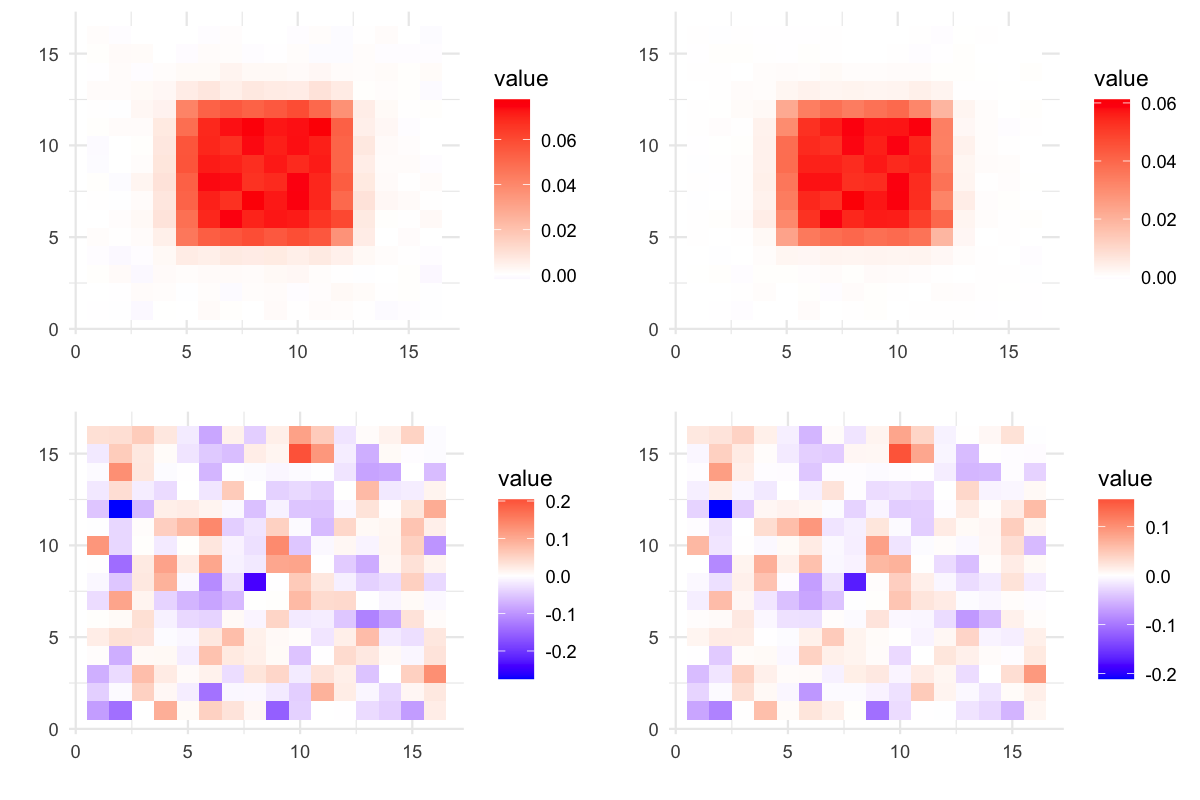
\includegraphics[width=0.9\textwidth]{beta_estimates.png} 
  \caption{Mean estimated \( \beta \) values across simulations, with models fitted using \texttt{lambda.min} (left) and
  \texttt{lambda.1se} (right). The top row shows results for Simulation 1, while the bottom row shows results for Simulation 2.}
	\label{fig:beta_estimates} 
\end{figure}

\begin{figure}[htbp] 
	\centering
  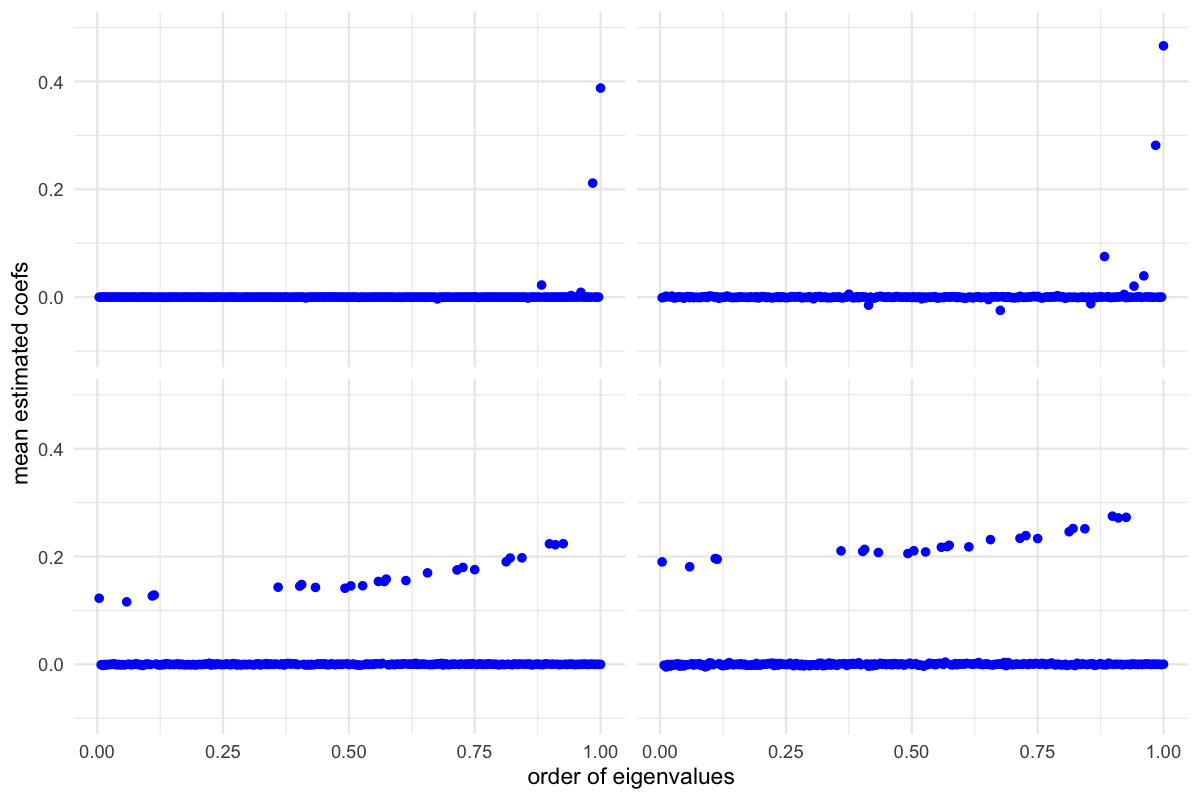
\includegraphics[width=0.9\textwidth]{b_estimates.png} 
  \caption{Mean estimated \( b \) values across simulations, plotted against ordered eigenvalues. Models fitted using
  \texttt{lambda.min} are on the left and models fitted with \texttt{lambda.1se} on the right. The top row shows results for Simulation 1, while the bottom row shows results for Simulation 2.}
  \label{fig:b_estimates} 
\end{figure}

Figure \ref{fig:perc_sign_beta} shows the percentage of significant elements in \( \beta \) when fitting models in the
pixel space for Simulation 1 (left) and Simulation 2 (right). A permutation test was performed, where the original
coefficient estimates were compared to those obtained after permuting the covariates 100 times. The p-value was
calculated as the proportion of times the absolute value of the original estimates exceeded those in the permutations.
The results indicate that, regardless of whether sparsity is assumed in the pixel space or frequency space, significant
p-values provide little information about the actual non-zero coefficients. Figure \ref{fig:perc_sign_b} shows the corresponding percentage of significant p-values of \( b \) across both
simulations, plotted against the order of eigenvalues. No clear pattern emerged, indicating that evaluating significance
based on p-values may not be effective for identifying meaningful pixels or frequencies.

\begin{figure}[htbp] 
	\centering
  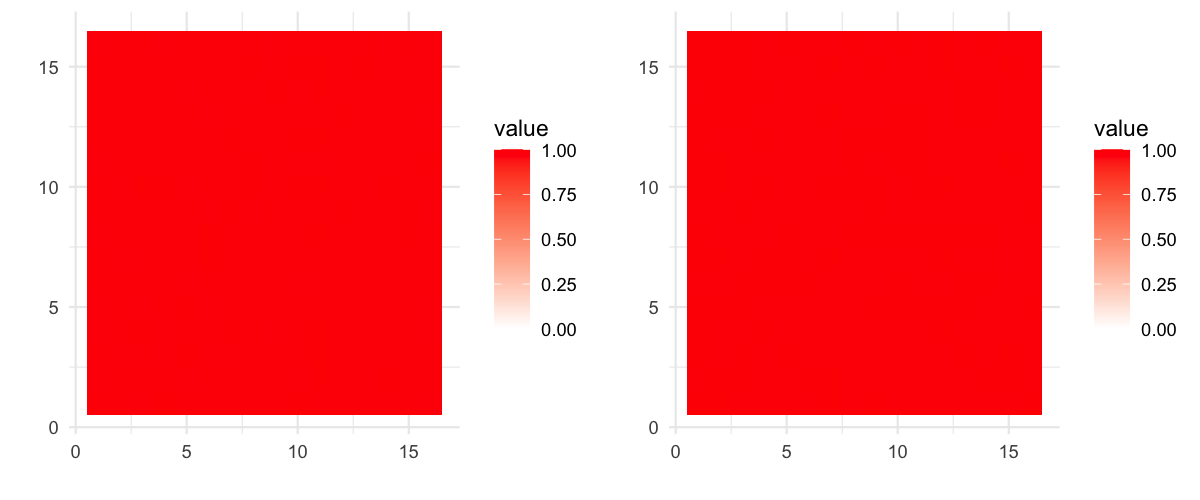
\includegraphics[width=0.9\textwidth]{perc_sign_pvals_beta.png} 
  \caption{Percentage of significant p-values for elements of \( \beta \) when fitting models in the pixel space in
  Simulation 1 (left) and Simulation 2 (right).}
	\label{fig:perc_sign_beta} 
\end{figure}

\begin{figure}[htbp] 
	\centering
  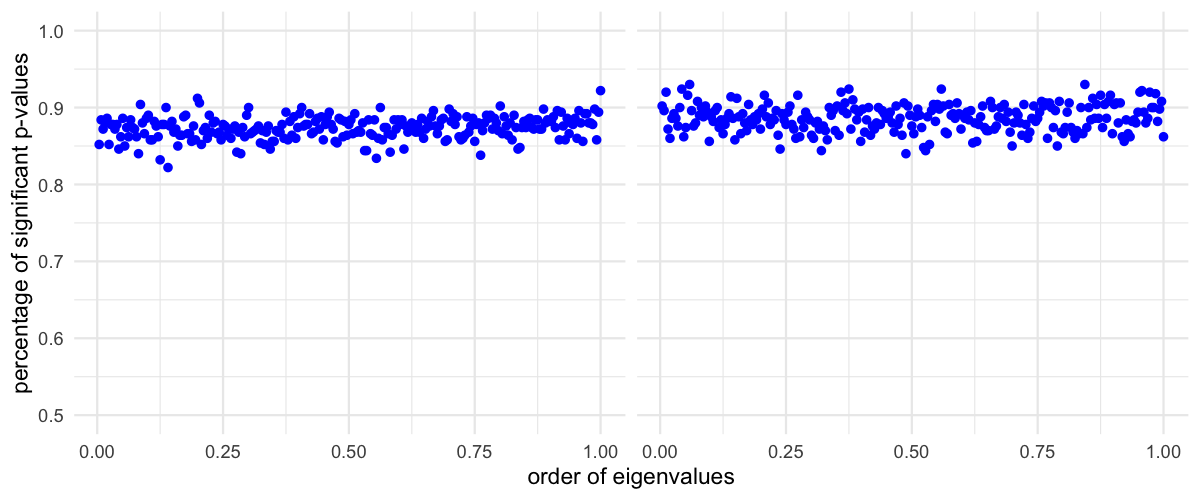
\includegraphics[width=0.9\textwidth]{perc_sign_pvals_b.png} 
  \caption{Percentage of significant p-values for elements of \( b \) across ordered eigenvalues in both simulations.}
	\label{fig:perc_sign_b} 
\end{figure}

Figure~\ref*{fig:top_bottom_eigvecs} presents the frequencies associated with the top three eigenvalues, which represent
the dominant patterns in the pixel space. The frequency associated with the smallest eigenvalue is also shown,
highlighting the least significant variance.

\begin{figure}[htbp] 
	\centering
	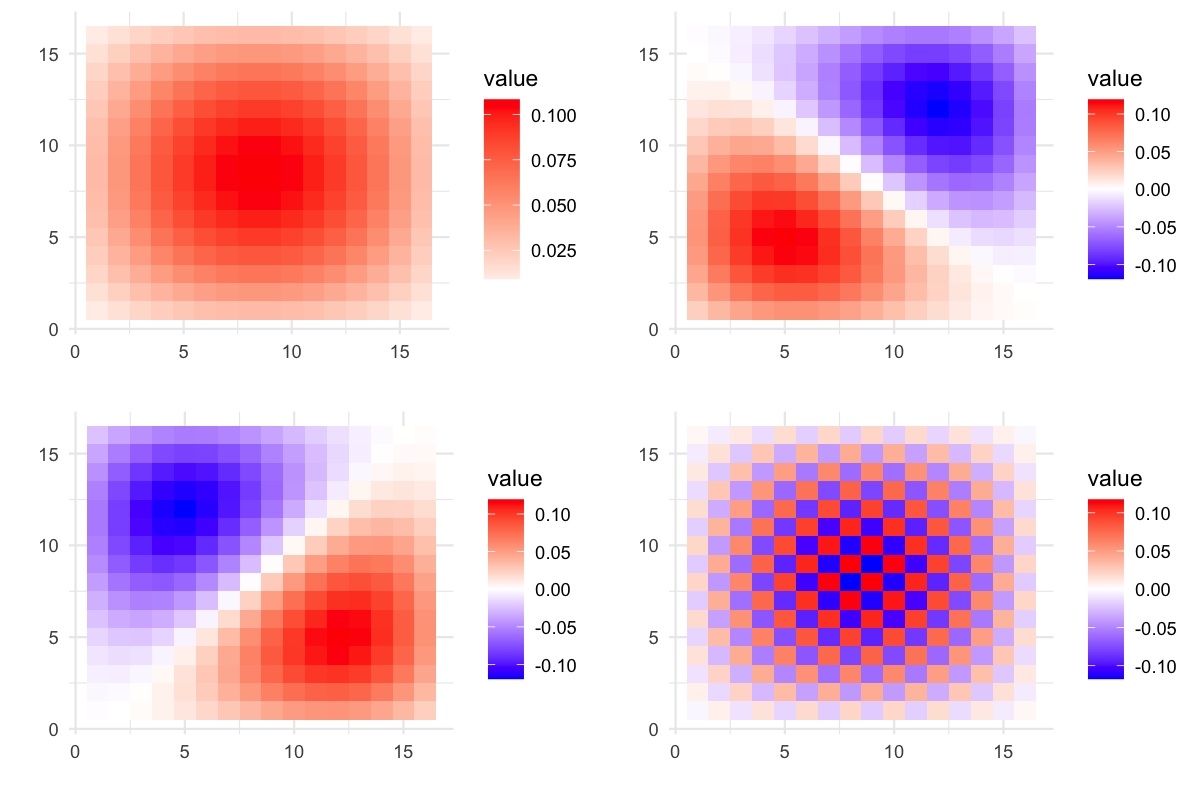
\includegraphics[width=0.8\textwidth]{top_bottom_eigvecs.png} 
\caption{Frequencies associated with the top three eigenvalues (top row and
bottom left) and the frequency associated with the smallest eigenvalue (bottom
right), highlighting the primary and least significant patterns in the pixel
space.}
	\label{fig:top_bottom_eigvecs} 
\end{figure}


\end{document}
